\documentclass[12pt,a4paper]{report}
\usepackage[utf8]{inputenc}
\usepackage[spanish]{babel}
\usepackage{amsmath}
\usepackage{amsfonts}
\usepackage{amssymb}
\usepackage{makeidx}
\usepackage{graphicx}
\usepackage[hidelinks]{hyperref}
\usepackage[left=2cm,right=2cm,top=2cm,bottom=2cm]{geometry}
\usepackage{hyperref}



\begin{document}

\author{Cesar Omar Alvarado Contreras\\
Marco Manzo Torrez\\
Eduardo Robles Vazquez\\
Victor Gabriel Tapia Casillas\\
Fonseca Camaarena Jonathan}

\title{\begin{center}

\includegraphics[scale=1.5]{Escudo.png} 
\end{center}Brazo Robótico Polar}

\date{
Universidad Politécnica de la Zona Metropolitana de Guadalajara\\
Profesor: Carlos Enrique Morán Garabito\\
19 de septiembre del 2019}

\maketitle
\tableofcontents
\section{Meta:}
Crear un robot polar de tres grados de libertad, con una longitud total de 50 centímetros y una altura total de 30 centímetros, cuyo último eslabón deberá soportar una carga de 500 gramos.
\section{Objetivos:}
\noindent
-Realizar boceto\\
-Cumplir con las especificaciones propuestas por el profesor\\
-Realizar el plano del robot\\
-Realizar el modelado del prototipo en 3D\\
-Establecer los materiales a usar\\ 
-Realizar el análisis de elementos finitos\\
-Realizar cálculos necesarios para la selección de motores y componentes\\
-Elaboración del primer prototipo\\
-Programación del robot\\



\section{Justificación}
El propósito de este proyecto surge a partir de la necesidad de implementar los conocimientos obtenidos de las materias presentes en este año, así como las materias de cuatrimestres pasados.
Retomando lo mencionado con anterioridad, se desarrollará un prototipo de un brazo robótico polar, el cual consistirá de 3 grados de libertad; dos movimientos rotacionales y uno prismático.

\section{Tabla de materias}
A continuación presentamos la tabla de materias que nos ayudarán en nuestro proyecto.\\
\begin{figure}
  \centering
    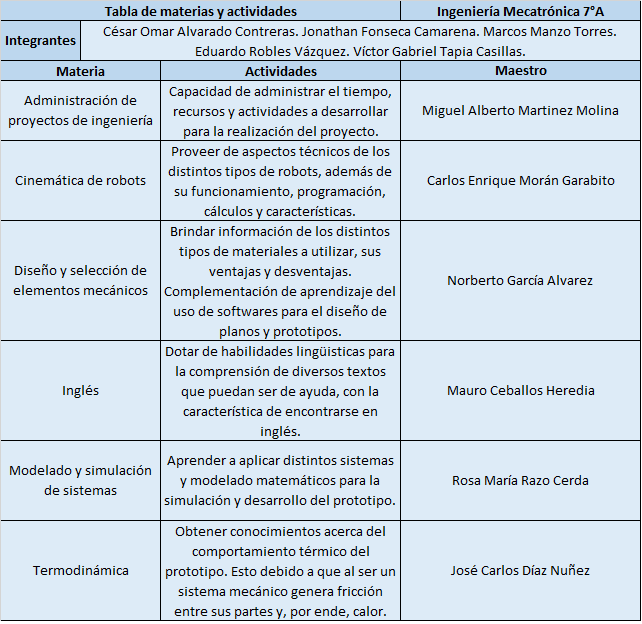
\includegraphics{Tabla.png}
  \caption{Tabla}
  \label{fig:Tabla}
\end{figure}


\section{Project}
En el programa Project realizamos el cronograma de actividades.\\

\centering
  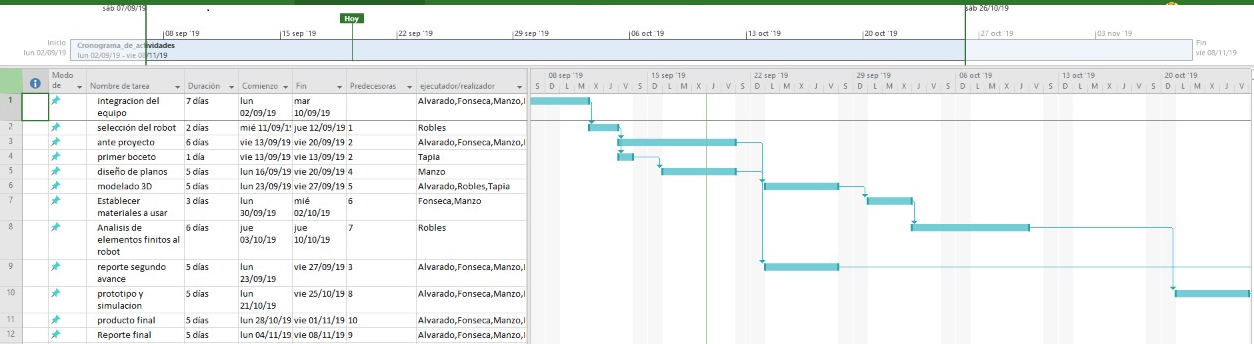
\includegraphics[scale=.5]{Project.png}\\
    Figura 2:Project
  


\section{Referencia}

  E.F. Morales and L.E. Sucar,Los Robots del Futuro y su Importancia para M\'exico, Komputer Sapiens,
  year{2009},pages{7-12}


\bibliographystyle{unsrt}
\bibliography{Morales.bib}




\begin{center}
Gracias.
\end{center}


\end{document}